\chapter{Results of learning with the 15 dof Amesim model}
\label{app:E}
This appendix shows the learning results of the 15 dof Amesim model on two distinct datasets $V022.22 - L3.47$ and $V025.00 - L6.94$. Except for the longitudinal total acceleration and jerk, all the learned kinematic signals match closely with the observed one. The most important conclusions about the results can be found in section \ref{s:complex_learning_results}.\\
It should be noted that Figure \ref{fig:app_deltaE} and \ref{fig:app_delta_dotE}  show the angle of the front wheel of the bicycle model. In order to obtain the steerwheelangle, this relation is linearised by the factor $Gs = 16.96$ which means that $\delta_{SWA} = Gs\cdot\delta_{front}$. Further Figure \ref{fig:app_convE} displays the convergence during the learning process and plots $\bm{f}_{rel}$ over the iterations. Figure \ref{fig:app_gradE} shows the absolute difference between the learned and observed features. In Figure \ref{fig:app_weightsE} the learning of the weighting factors towards the final ones are presented. Figure \ref{fig:app_updateE} gives the difference of current weighting factors with respect to the previous one and as last Figure \ref{fig:app_multigradE} shows which of the three RPROP cases is used in order to update a certain weight factor.



\begin{figure}[h!]
	\centering
	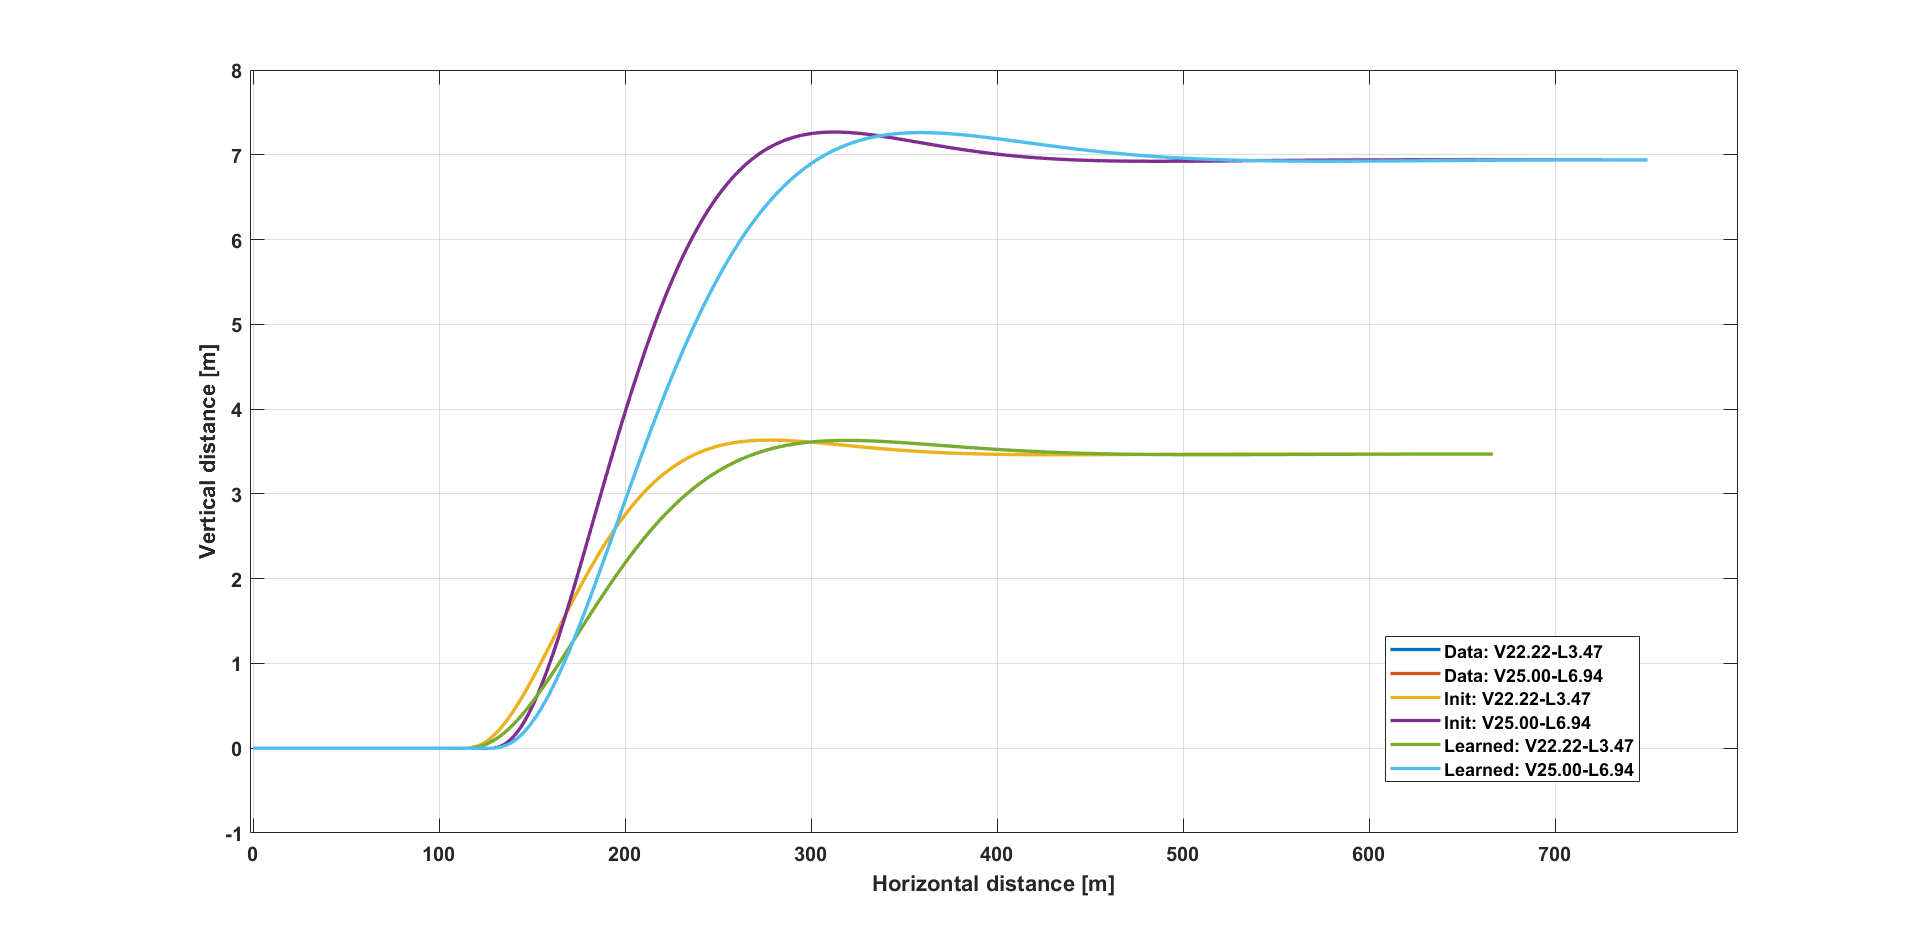
\includegraphics[width=1.15\textwidth]{2path_N1000IT28.PNG}
\end{figure}

\begin{figure}[h!]
	\centering
	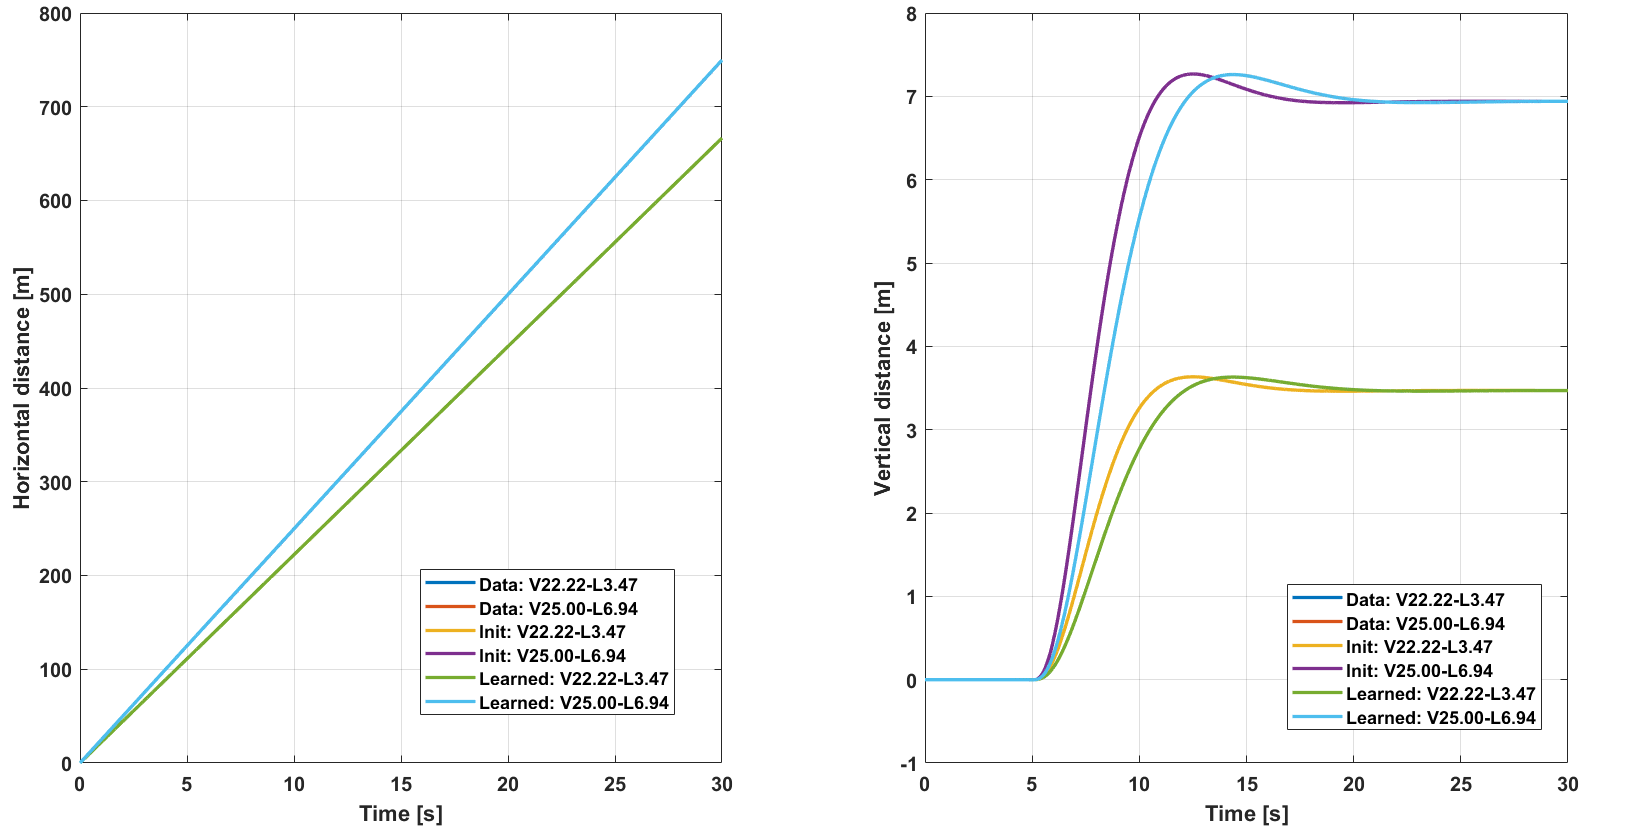
\includegraphics[width=1.15\textwidth]{1X_Y_N1000IT28.PNG}
\end{figure}


\begin{figure}[h!]
	\centering
	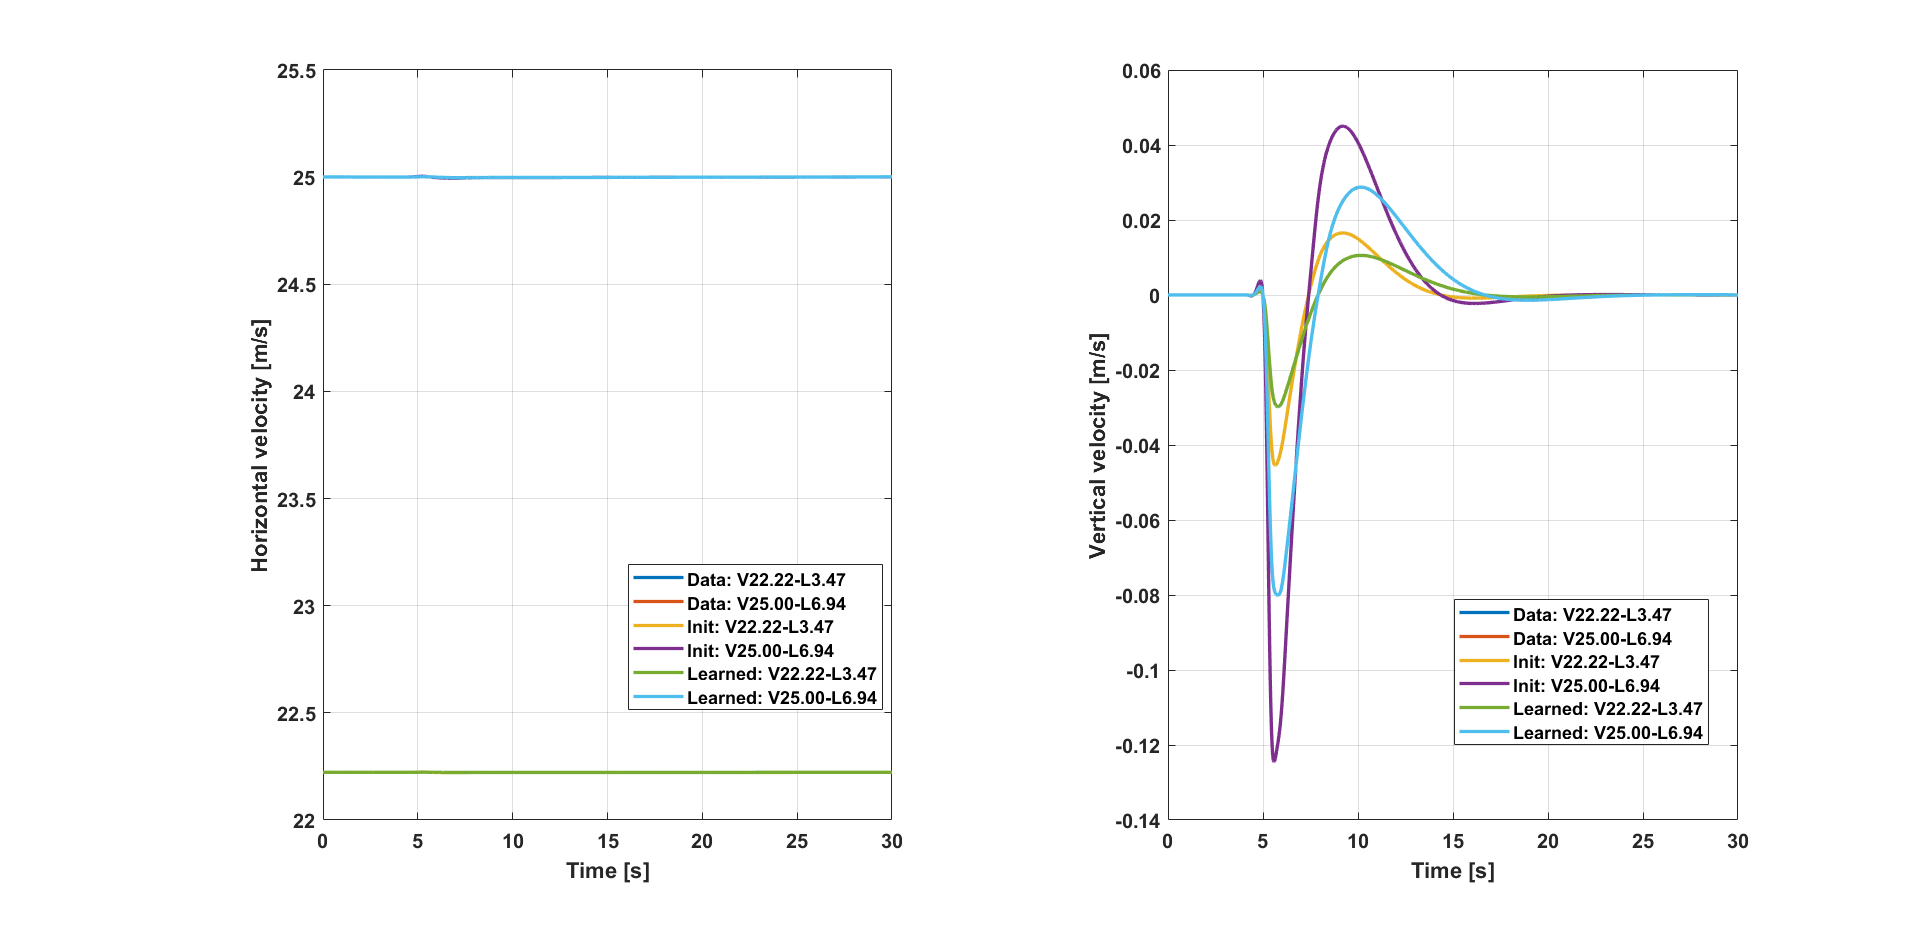
\includegraphics[width=1.15\textwidth]{3VX_VY_N1000IT28.PNG}
\end{figure}


\begin{figure}[h!]
	\centering
	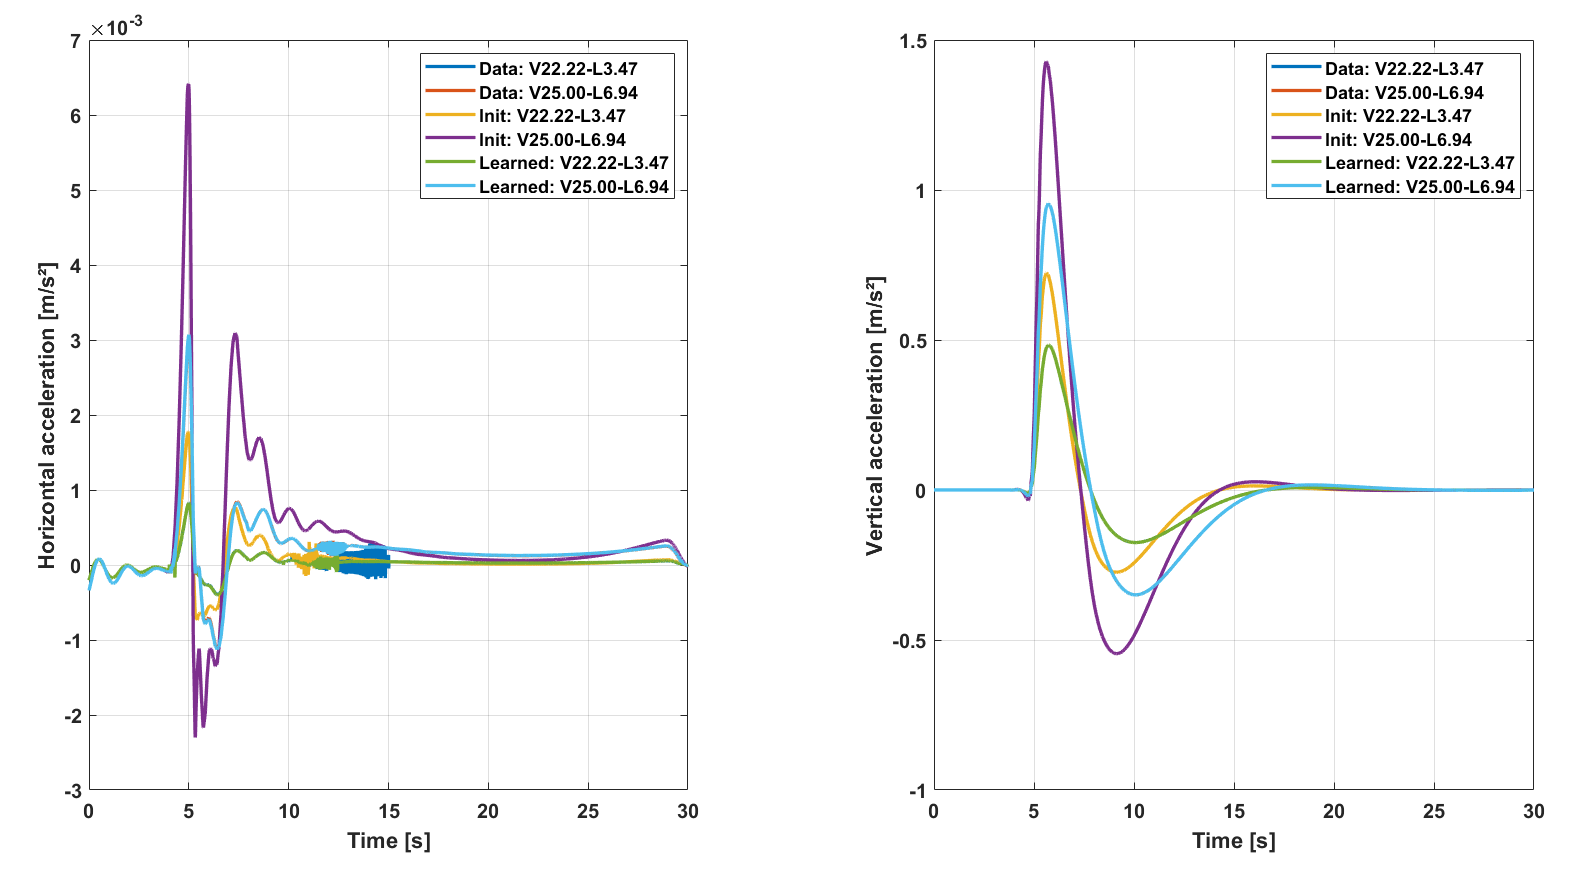
\includegraphics[width=1.15\textwidth]{4AX_AY_N1000IT28.PNG}
\end{figure}


\begin{figure}[h!]
	\centering
	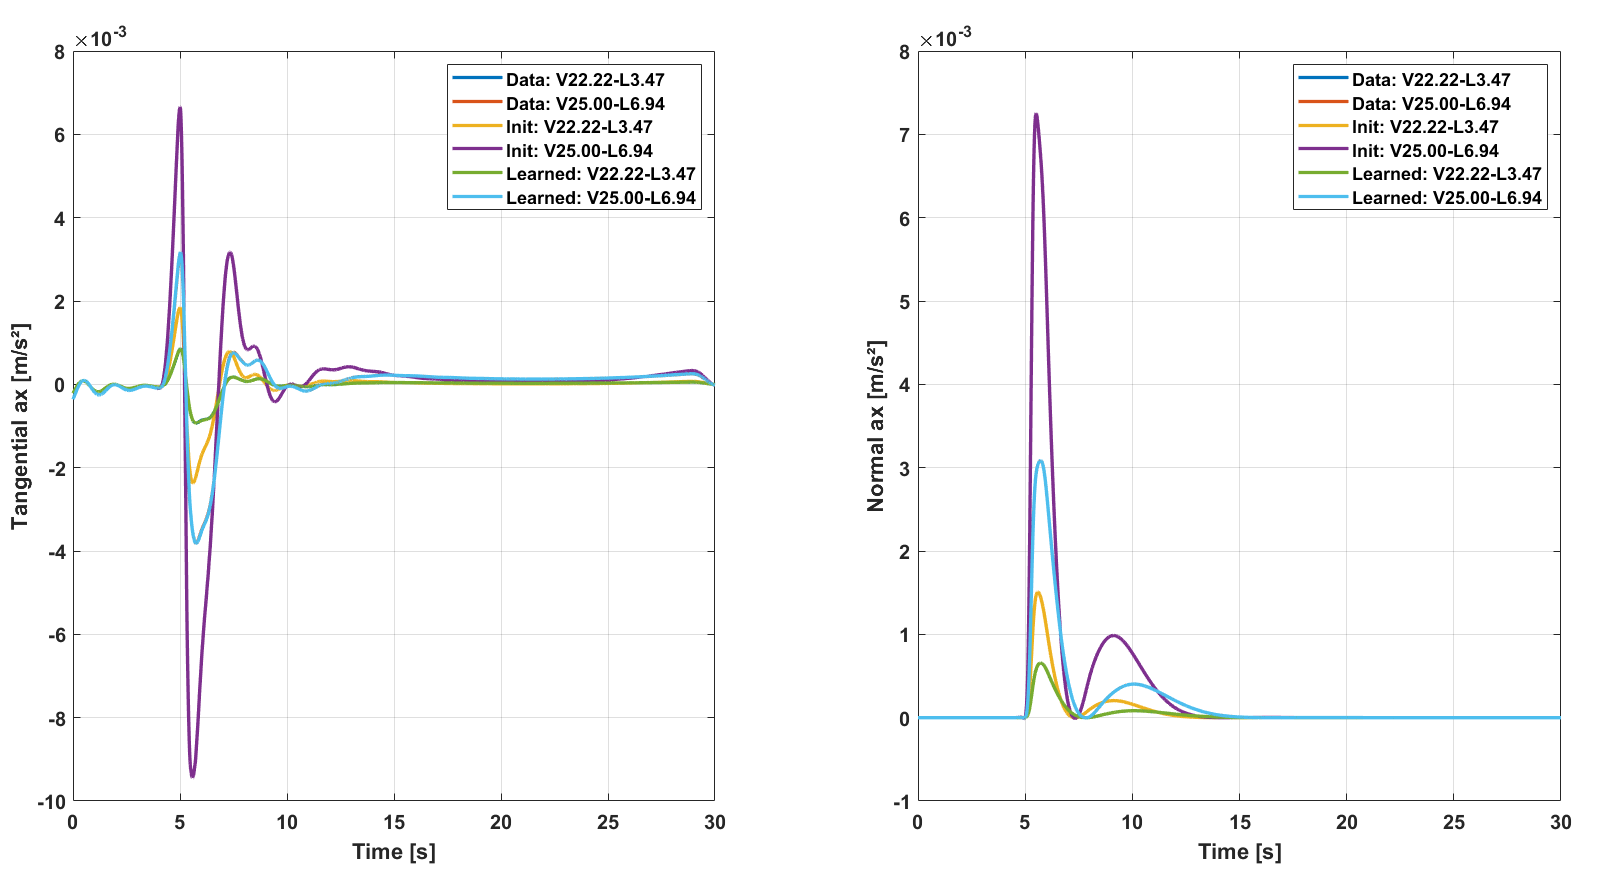
\includegraphics[width=1.15\textwidth]{5AtX_AnX_N1000IT28.PNG}
\end{figure}

\begin{figure}[h!]
	\centering
	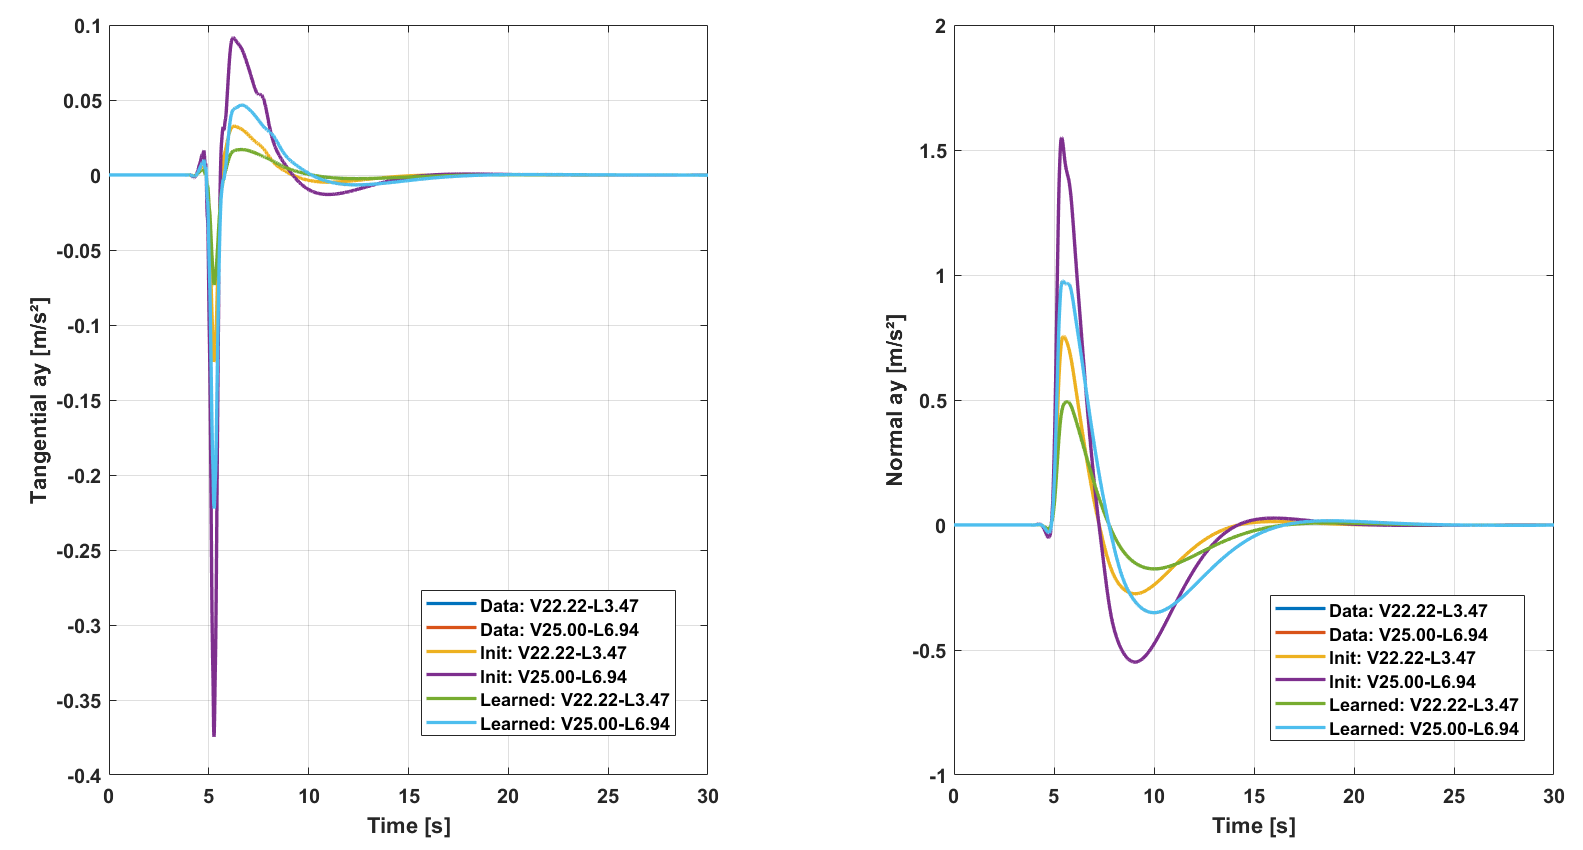
\includegraphics[width=1.15\textwidth]{6AtY_AnY_N1000IT28.PNG}
\end{figure}

\begin{figure}[h!]
	\centering
	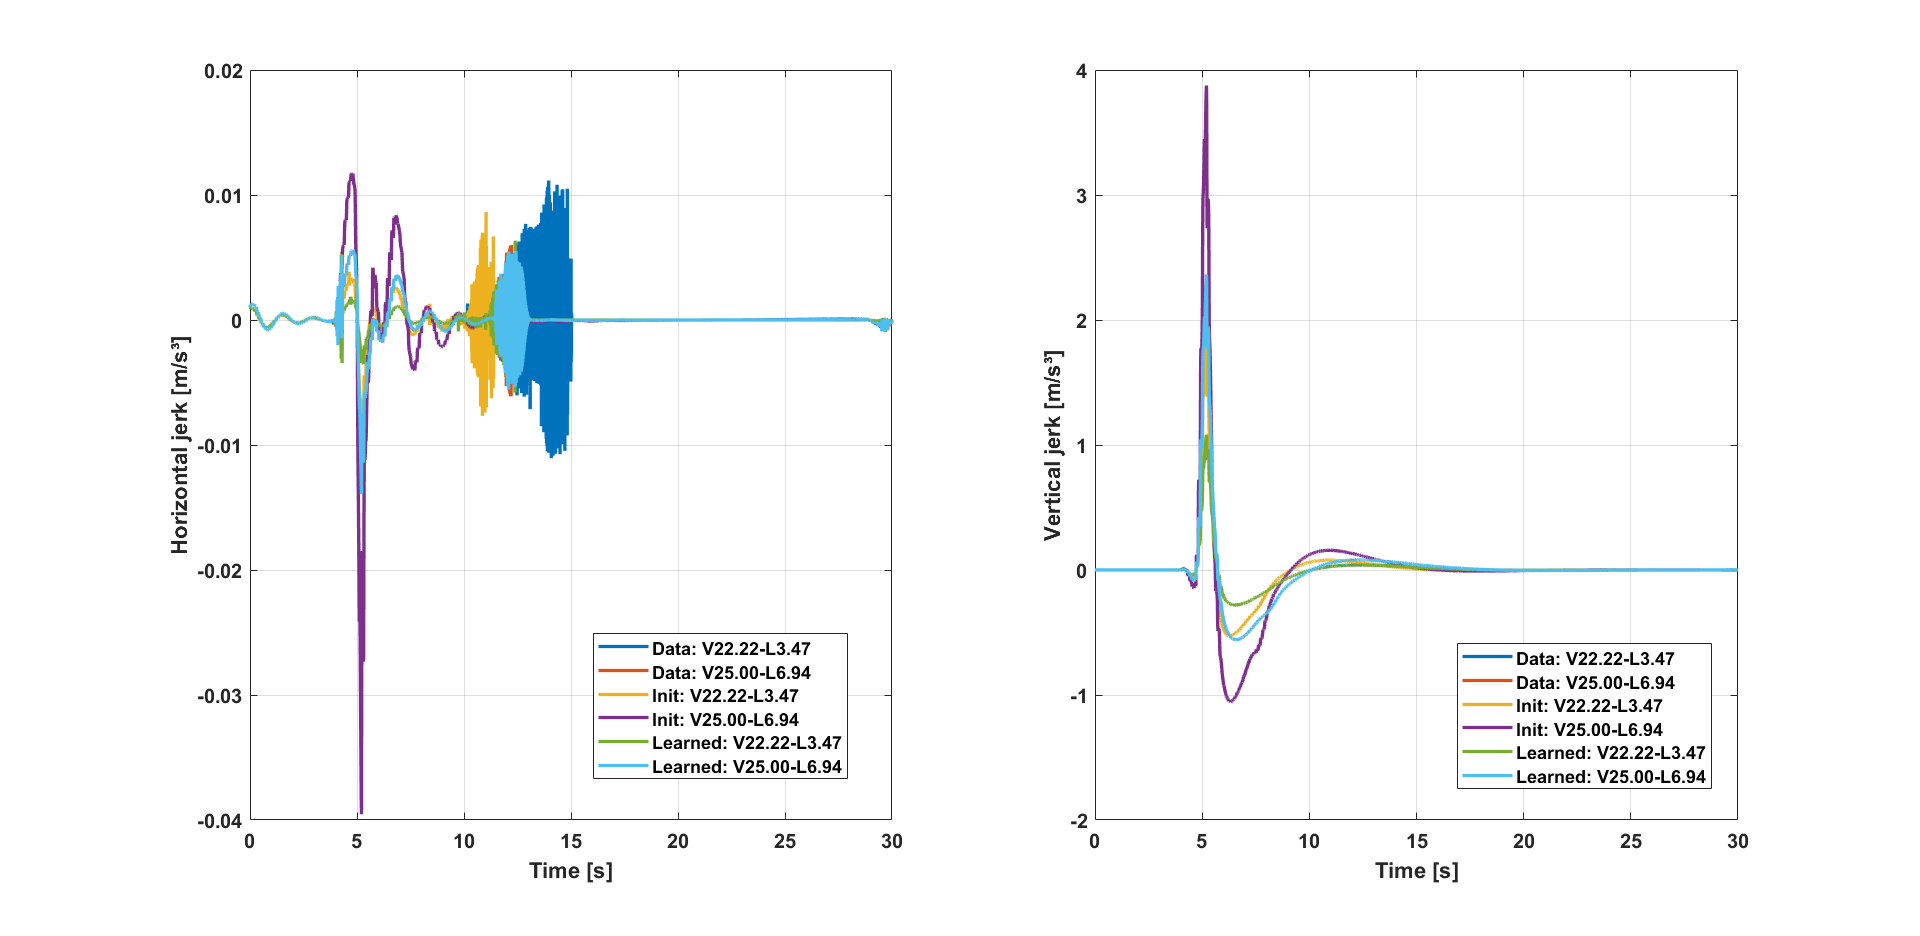
\includegraphics[width=1.15\textwidth]{7JX_JY_N1000IT28.PNG}
\end{figure}

\begin{figure}[h!]
	\centering
	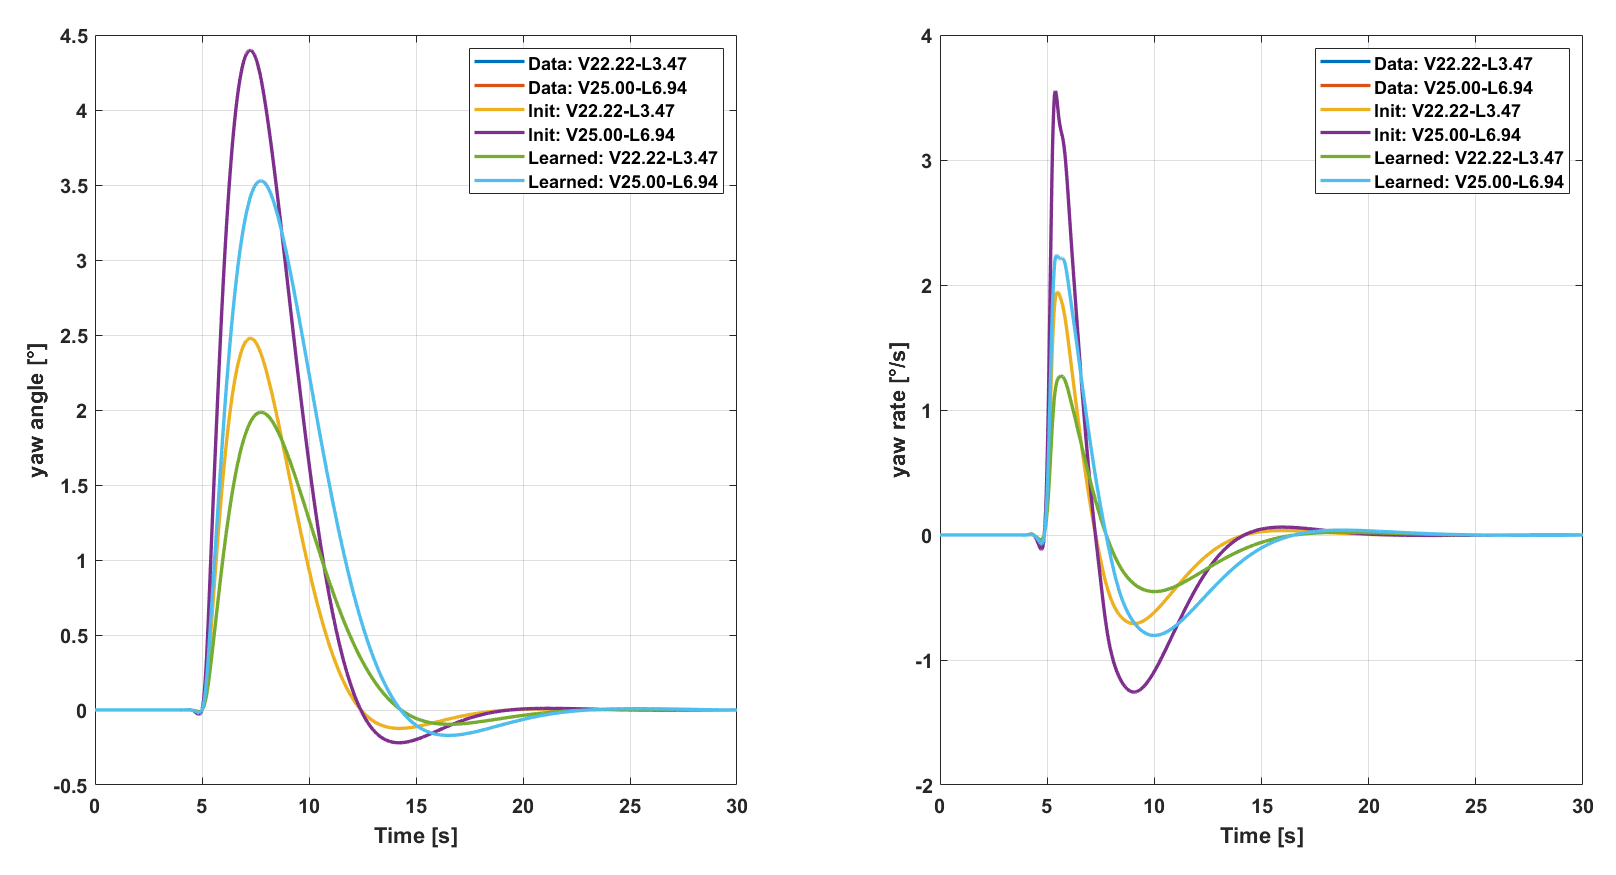
\includegraphics[width=1.15\textwidth]{8yaws_N1000IT28.PNG}
\end{figure}

\begin{figure}[h!]
	\centering
	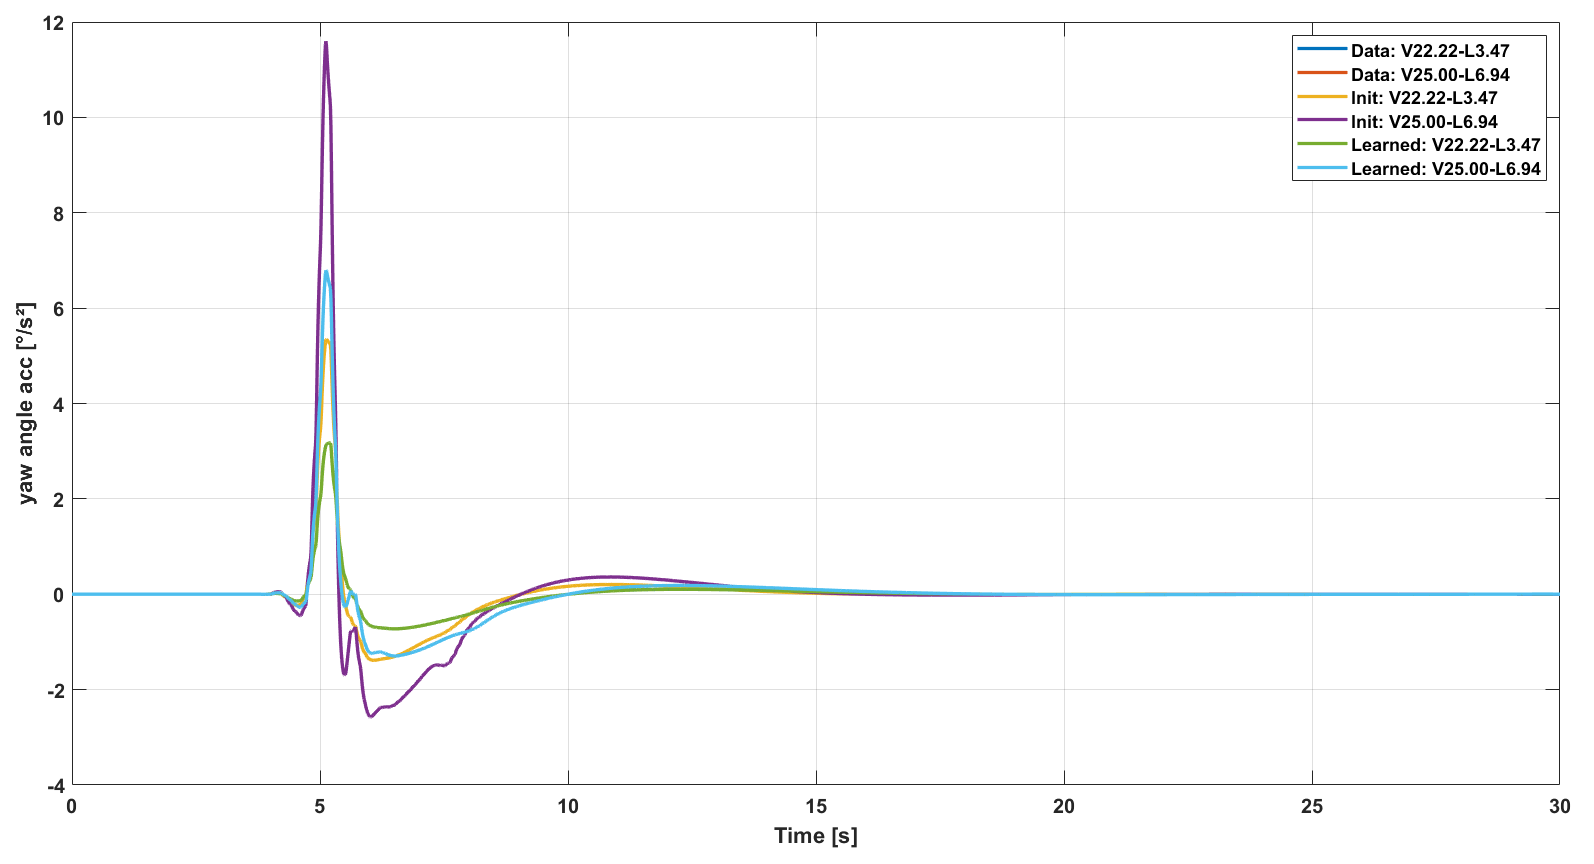
\includegraphics[width=1.15\textwidth]{9yawacc_N1000IT28.PNG}
\end{figure}

\begin{figure}[h!]
	\centering
	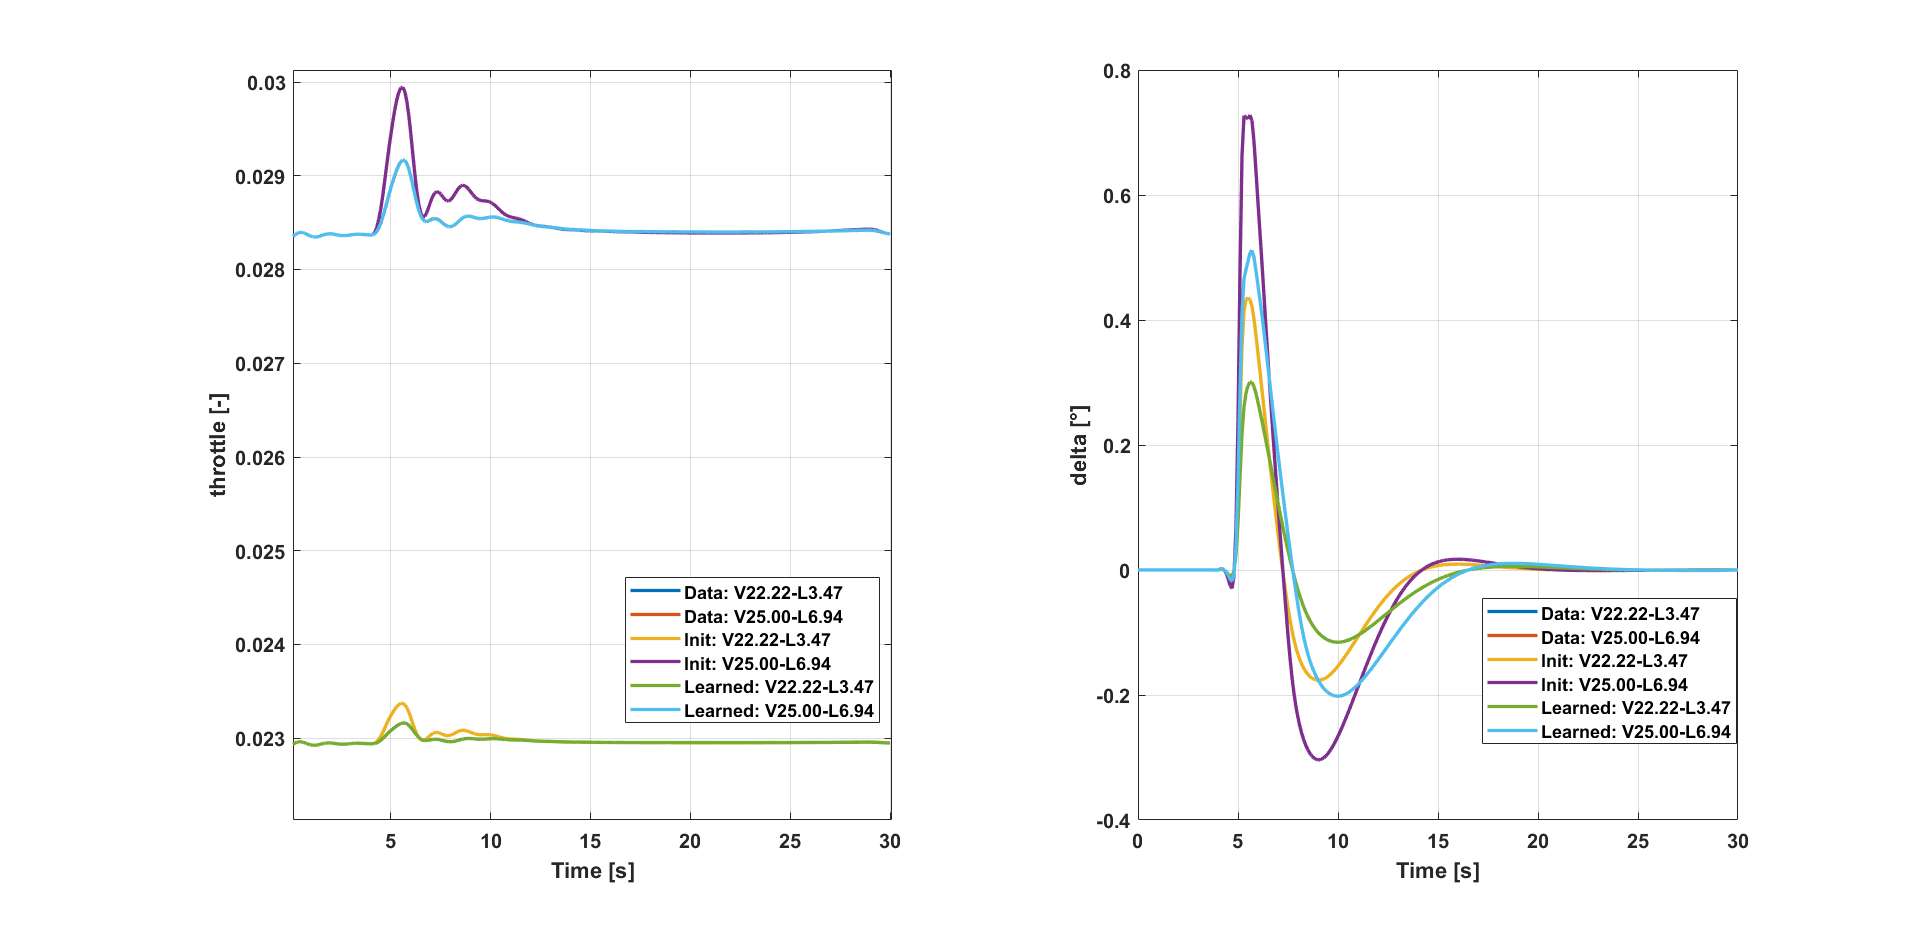
\includegraphics[width=1.15\textwidth]{10trdelta_N1000IT28.PNG}
	\caption{This figure shows the amount of throttle and the angle of the front wheel of the bicycle model during the lane change maneuvers.}
	\label{fig:app_deltaE}
\end{figure}

\begin{figure}[h!]
	\centering
	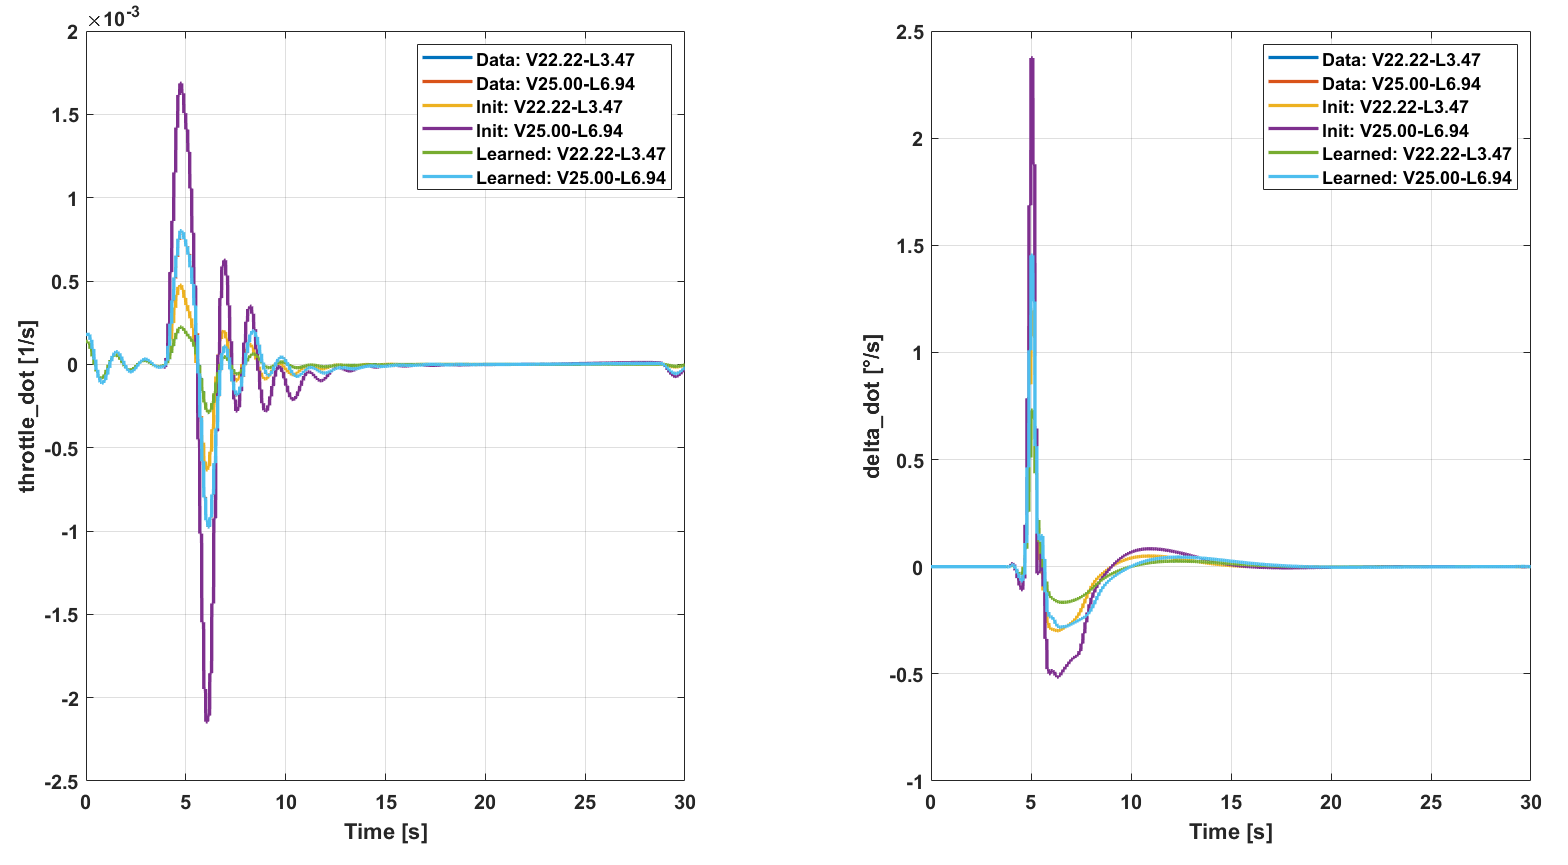
\includegraphics[width=1.15\textwidth]{11trdelta_dot_N1000IT28.PNG}
	\caption{This figure shows the amount of first derivative of throttle and the first derivative of the angle of the front wheel of the bicycle model is given as input during the lane change maneuvers.}
	\label{fig:app_delta_dotE}
\end{figure}

\begin{figure}[h!]
	\centering
	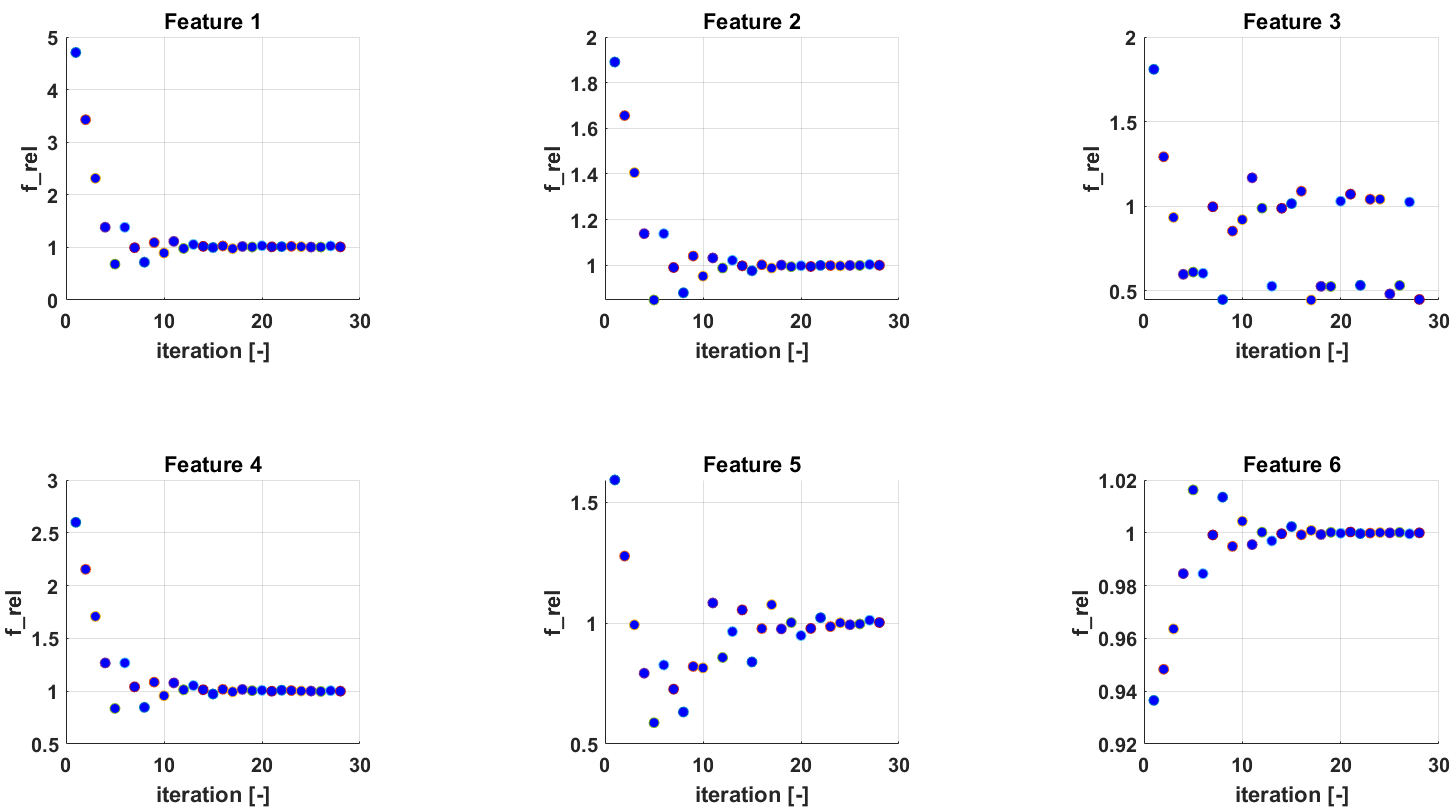
\includegraphics[width=1.15\textwidth]{12frel.PNG}
	\caption{The convergence of $\bm{f}_{rel}$ towards one during the learning iterations.}
	\label{fig:app_convE}
\end{figure}

\begin{figure}[h!]
	\centering
	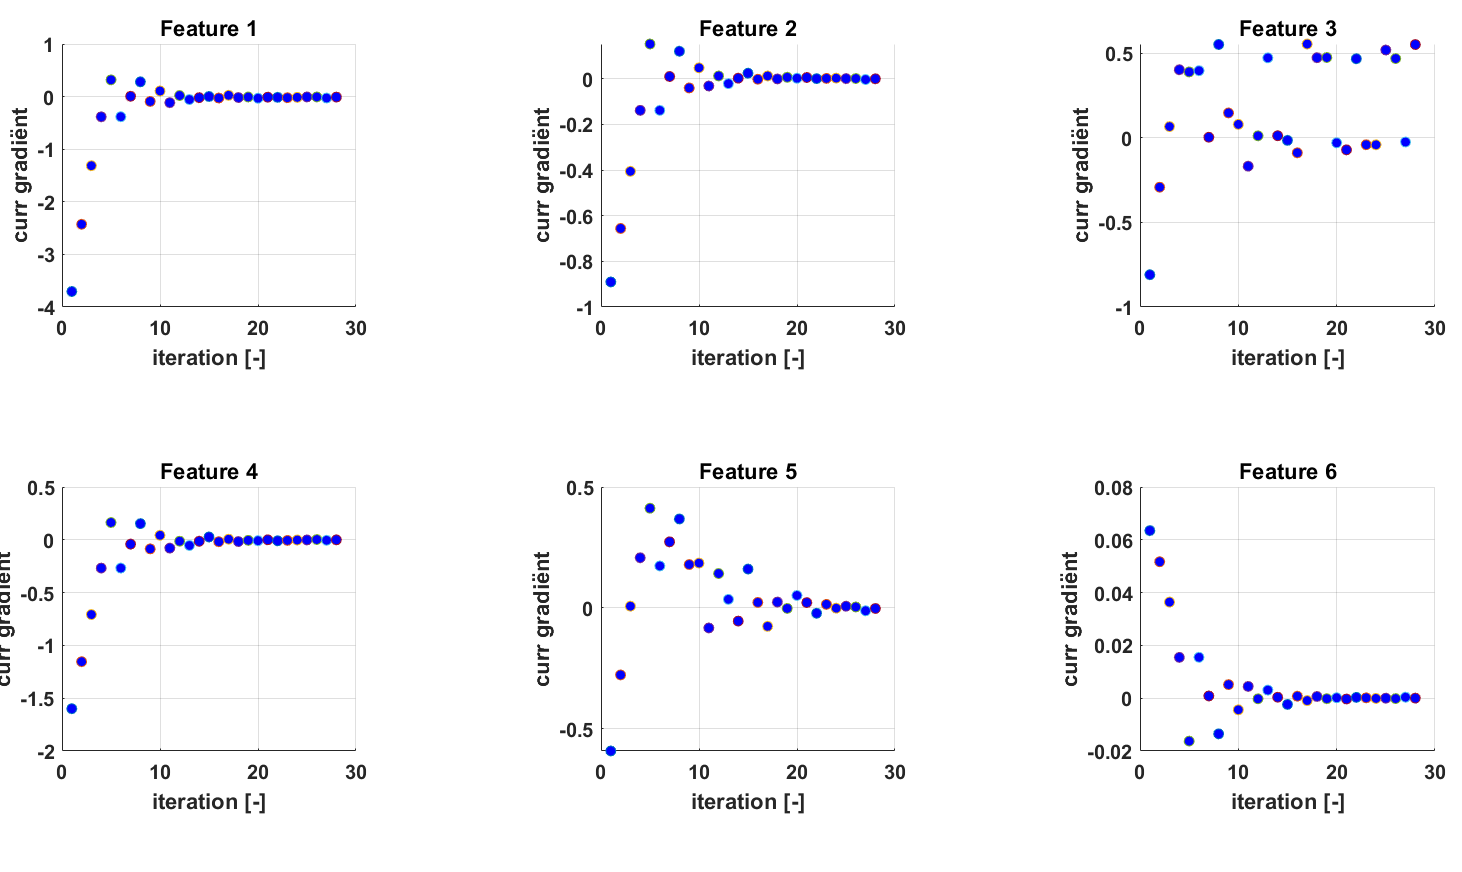
\includegraphics[width=1.15\textwidth]{13gradcurr.PNG}
	\caption{The gradient $\pdv{\bm{F}}{\bm{\theta}}$ estimated by $\bm{F}_{obs} - \bm{F}(\bm{r}_{expected})$ towards zero during the different learning iterations. }
	\label{fig:app_gradE}
\end{figure}

\begin{figure}[h!]
	\centering
	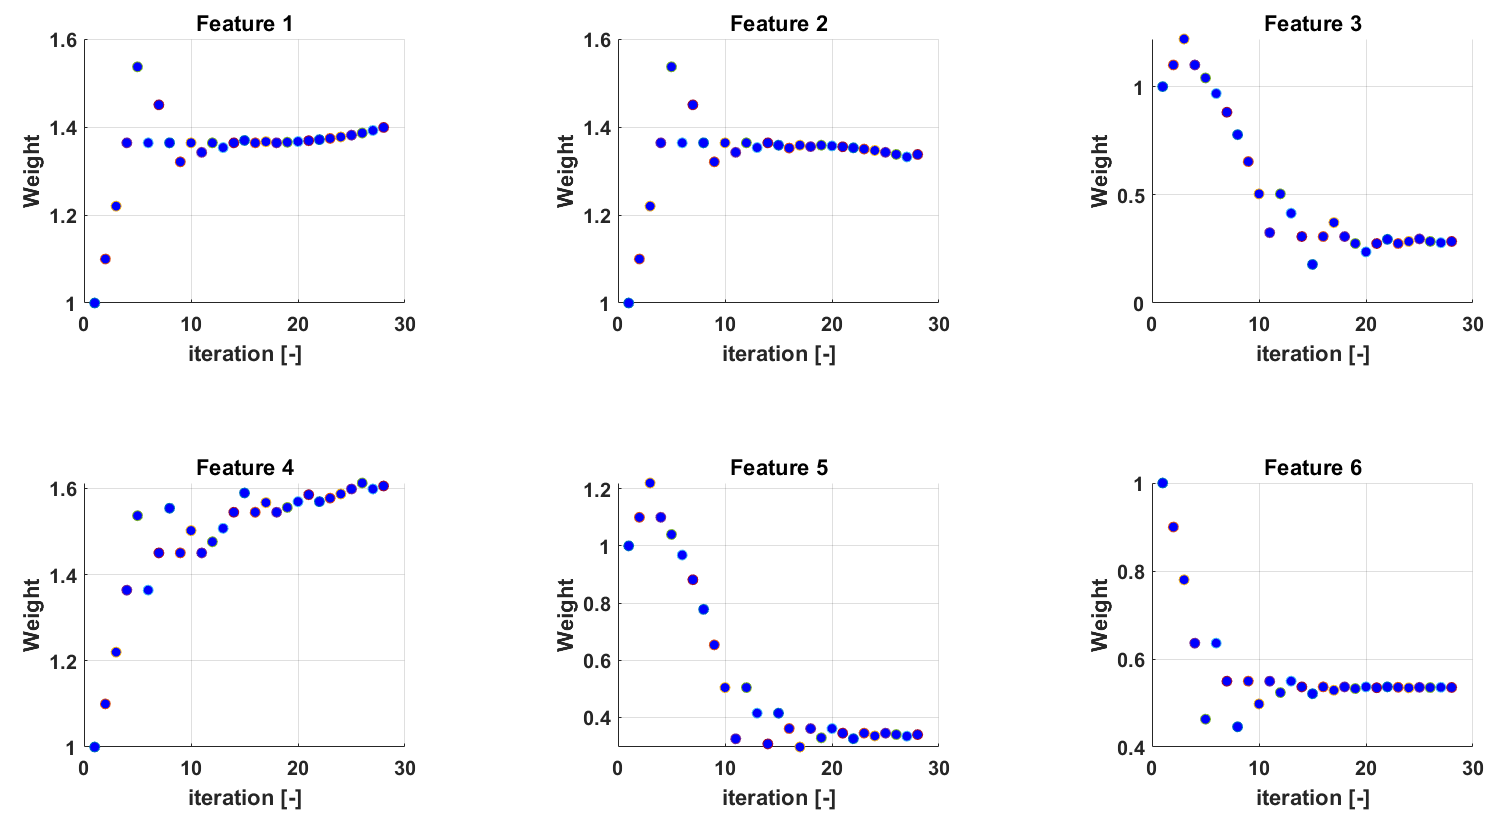
\includegraphics[width=1.15\textwidth]{14weights.PNG}
	\caption{The learned weighting factors during the different learning iterations.}
	\label{fig:app_weightsE}
\end{figure}

\begin{figure}[h!]
	\centering
	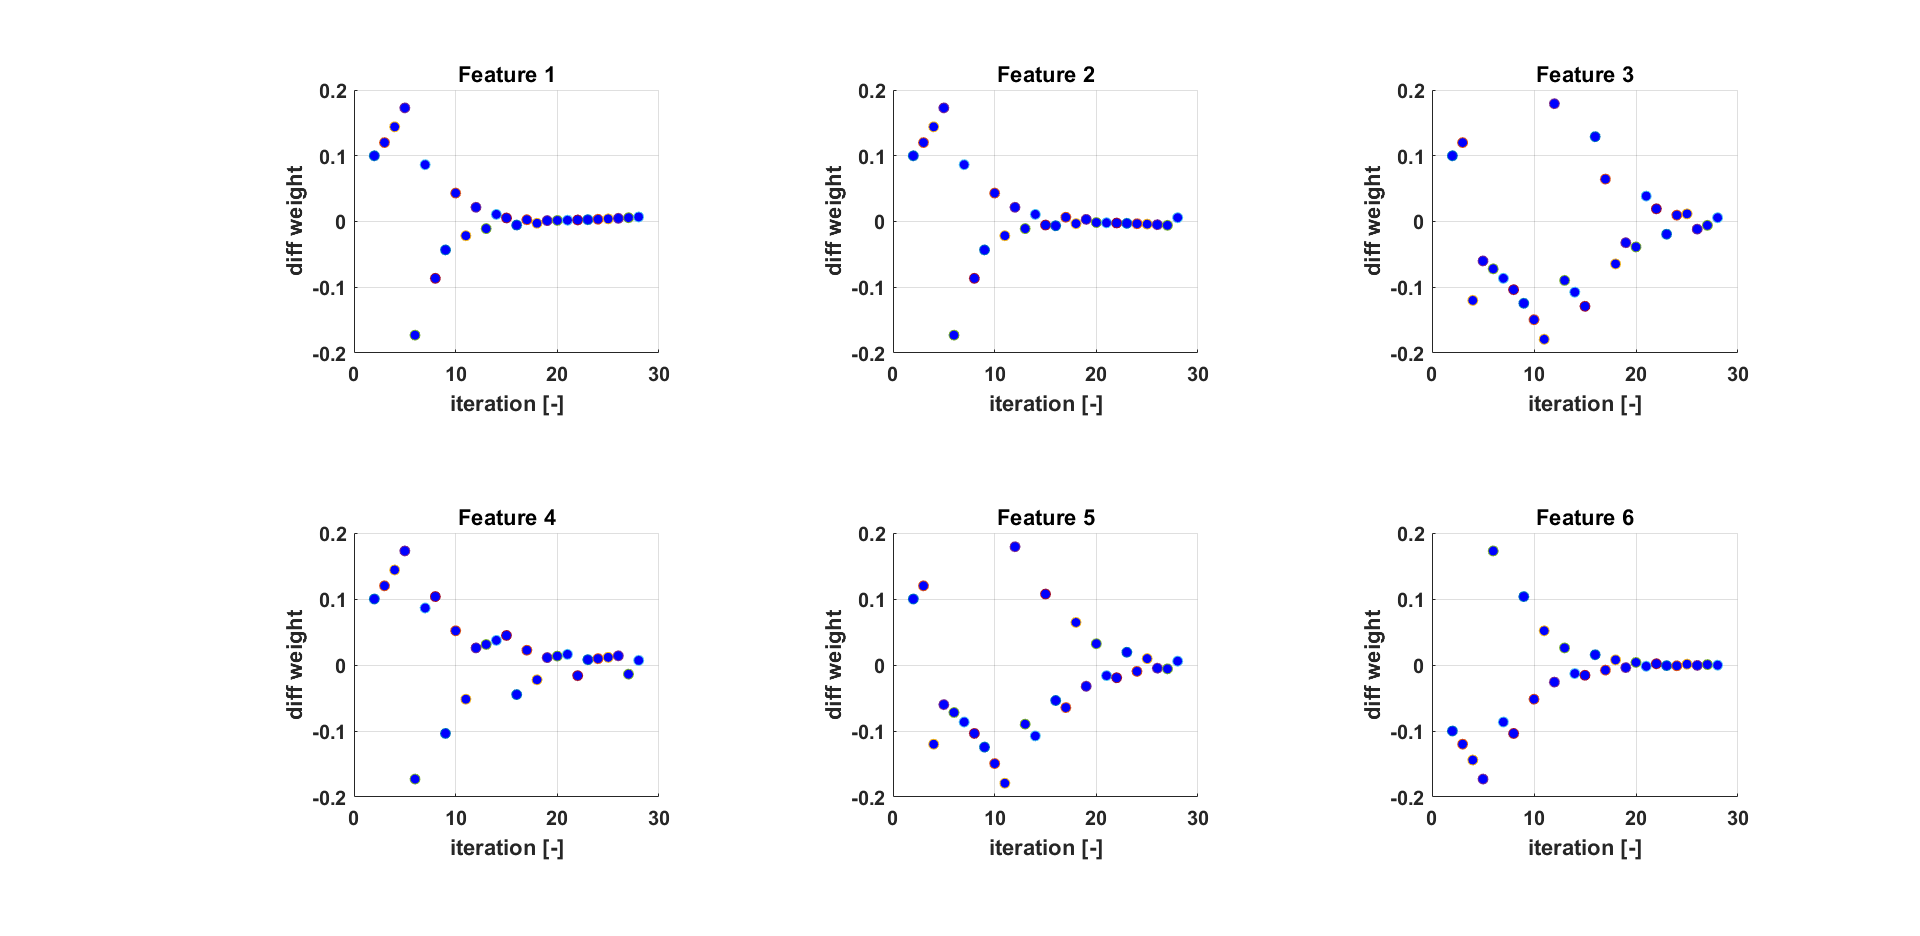
\includegraphics[width=1.15\textwidth]{15updateweights.PNG}
	\caption{The difference of $\bm{\theta}$ with respect to one used in the previous iteration. }
	\label{fig:app_updateE}
\end{figure}

\begin{figure}[h!]
	\centering
	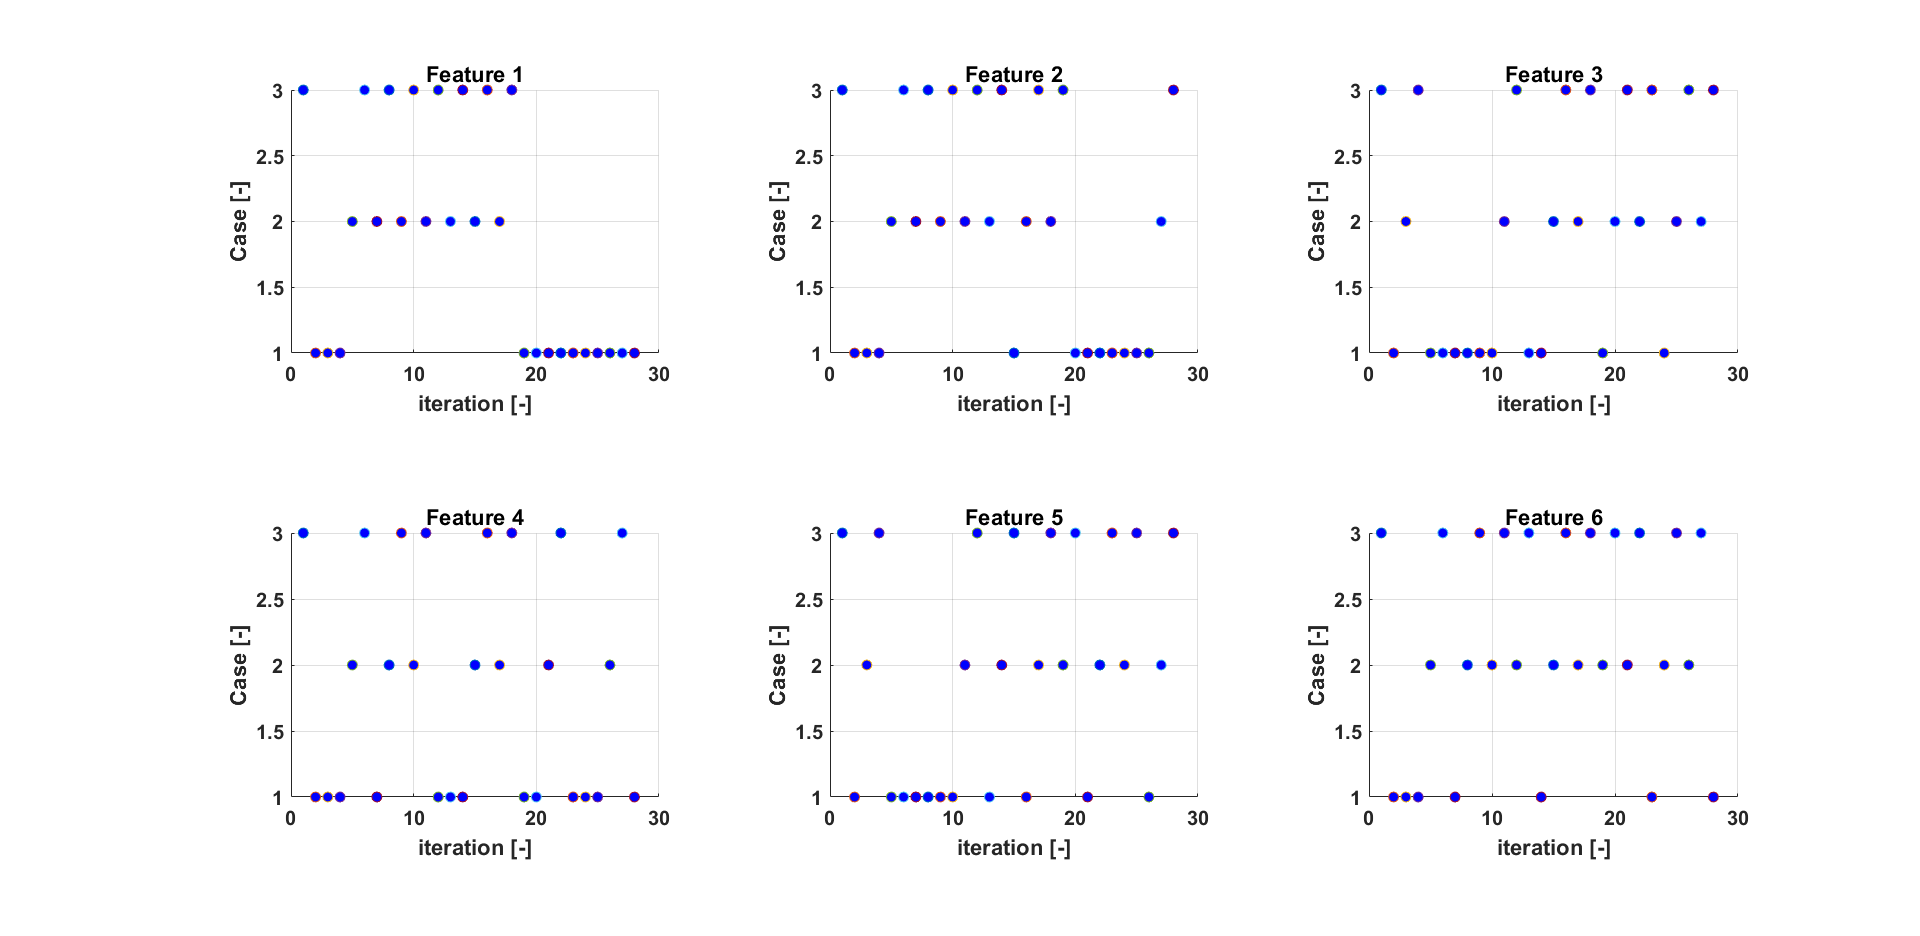
\includegraphics[width=1.15\textwidth]{16multigrad.PNG}
	\caption{This figure shows which case of the three available in the RPROP algorithm is chosen during the learning iterations.}
	\label{fig:app_multigradE}
\end{figure}





%%% Local Variables: 
%%% mode: latex
%%% TeX-master: "thesis"
%%% End: 
